\documentclass[border=10pt]{standalone}
\usepackage{fontspec}
\setmainfont{Carlito}
\setsansfont{Carlito}
\usepackage{tikz}
\usepackage{xcolor}
\usetikzlibrary{positioning, calc}

\definecolor{canvabg}{RGB}{246,244,241}
\pagecolor{canvabg}

\definecolor{meetgreen}{RGB}{80,160,100}
\definecolor{partamber}{RGB}{210,170,60}
\definecolor{failred}{RGB}{200,90,80}
\definecolor{rowgrey}{RGB}{238,234,228}        % warm tint of canvabg
\definecolor{headblue}{RGB}{70,130,180}
\definecolor{neutralgrey}{RGB}{80,80,90}
\definecolor{highlightgreen}{RGB}{222,240,225}  % softer, warmer green
\definecolor{linegrey}{RGB}{200,195,188}        % warmer rule colour

% Stroke widths (bolder presentation feel)
\def\circStroke{1.1pt}
\def\rowStroke{1.0pt}
\def\sepStroke{1.4pt}

\begin{document}
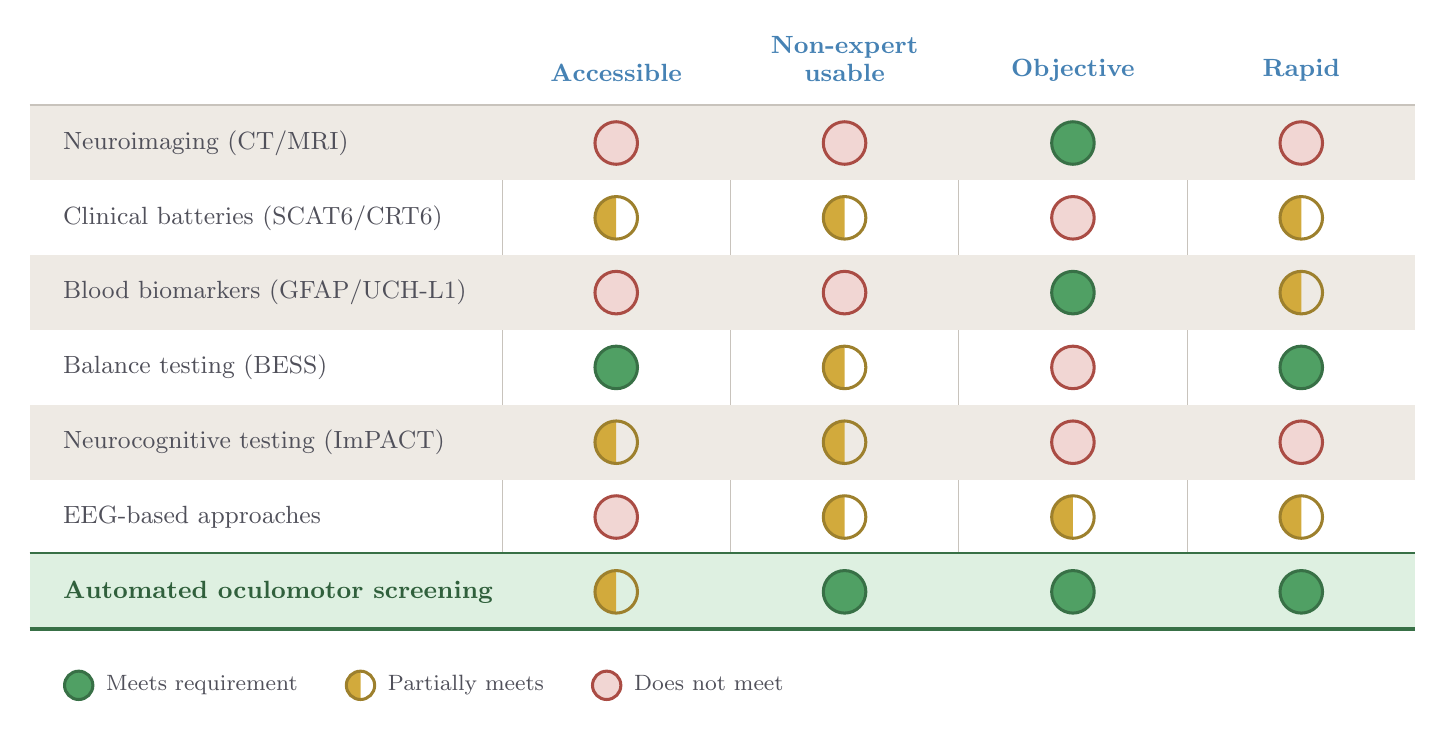
\begin{tikzpicture}[every node/.style={font=\sffamily}]

% Grid dimensions
\def\colw{2.9cm}
\def\rowh{0.95cm}
\def\labelw{6.0cm}
\def\circr{0.27cm}

% Column headers
\node[anchor=south, font=\small\bfseries, text=headblue, align=center, text width=\colw]
  at (\labelw + 0.5*\colw, 0.18) {Accessible};
\node[anchor=south, font=\small\bfseries, text=headblue, align=center, text width=\colw]
  at (\labelw + 1.5*\colw, 0.18) {Non-expert\\[-1pt]usable};
\node[anchor=south, font=\small\bfseries, text=headblue, align=center, text width=\colw]
  at (\labelw + 2.5*\colw, 0.18) {Objective};
\node[anchor=south, font=\small\bfseries, text=headblue, align=center, text width=\colw]
  at (\labelw + 3.5*\colw, 0.18) {Rapid};

% Header line
\draw[linegrey, line width=\rowStroke] (0,0) -- (\labelw + 4*\colw,0);

% Vertical column separators
\foreach \i in {0,1,2,3} {
  \draw[linegrey, line width=0.4pt] (\labelw + \i*\colw, 0) -- (\labelw + \i*\colw, -6*\rowh);
}

% Helper macros for circles
\newcommand{\circMeet}[2]{%
  \fill[meetgreen] (#1, #2) circle (\circr);
  \draw[meetgreen!70!black, line width=\circStroke] (#1, #2) circle (\circr);
}
\newcommand{\circPart}[2]{%
  \begin{scope}
    \clip (#1 - \circr, #2 - \circr) rectangle (#1, #2 + \circr);
    \fill[partamber] (#1, #2) circle (\circr);
  \end{scope}
  \draw[partamber!75!black, line width=\circStroke] (#1, #2) circle (\circr);
}
\newcommand{\circFail}[2]{%
  \fill[failred!25] (#1, #2) circle (\circr);
  \draw[failred!85!black, line width=\circStroke] (#1, #2) circle (\circr);
}

% --- Row 1: Neuroimaging (shaded) ---
\fill[rowgrey] (0, -\rowh) rectangle (\labelw + 4*\colw, 0);
\node[anchor=west, font=\small, text=neutralgrey] at (0.3, -0.5*\rowh) {Neuroimaging (CT/MRI)};
\circFail{\labelw + 0.5*\colw}{-0.5*\rowh}
\circFail{\labelw + 1.5*\colw}{-0.5*\rowh}
\circMeet{\labelw + 2.5*\colw}{-0.5*\rowh}
\circFail{\labelw + 3.5*\colw}{-0.5*\rowh}

% --- Row 2: Clinical batteries ---
\node[anchor=west, font=\small, text=neutralgrey] at (0.3, -1.5*\rowh) {Clinical batteries (SCAT6/CRT6)};
\circPart{\labelw + 0.5*\colw}{-1.5*\rowh}
\circPart{\labelw + 1.5*\colw}{-1.5*\rowh}
\circFail{\labelw + 2.5*\colw}{-1.5*\rowh}
\circPart{\labelw + 3.5*\colw}{-1.5*\rowh}

% --- Row 3: Blood biomarkers (shaded) ---
\fill[rowgrey] (0, -3*\rowh) rectangle (\labelw + 4*\colw, -2*\rowh);
\node[anchor=west, font=\small, text=neutralgrey] at (0.3, -2.5*\rowh) {Blood biomarkers (GFAP/UCH-L1)};
\circFail{\labelw + 0.5*\colw}{-2.5*\rowh}
\circFail{\labelw + 1.5*\colw}{-2.5*\rowh}
\circMeet{\labelw + 2.5*\colw}{-2.5*\rowh}
\circPart{\labelw + 3.5*\colw}{-2.5*\rowh}

% --- Row 4: Balance testing ---
\node[anchor=west, font=\small, text=neutralgrey] at (0.3, -3.5*\rowh) {Balance testing (BESS)};
\circMeet{\labelw + 0.5*\colw}{-3.5*\rowh}
\circPart{\labelw + 1.5*\colw}{-3.5*\rowh}
\circFail{\labelw + 2.5*\colw}{-3.5*\rowh}
\circMeet{\labelw + 3.5*\colw}{-3.5*\rowh}

% --- Row 5: Neurocognitive (shaded) ---
\fill[rowgrey] (0, -5*\rowh) rectangle (\labelw + 4*\colw, -4*\rowh);
\node[anchor=west, font=\small, text=neutralgrey] at (0.3, -4.5*\rowh) {Neurocognitive testing (ImPACT)};
\circPart{\labelw + 0.5*\colw}{-4.5*\rowh}
\circPart{\labelw + 1.5*\colw}{-4.5*\rowh}
\circFail{\labelw + 2.5*\colw}{-4.5*\rowh}
\circFail{\labelw + 3.5*\colw}{-4.5*\rowh}

% --- Row 6: EEG ---
\node[anchor=west, font=\small, text=neutralgrey] at (0.3, -5.5*\rowh) {EEG-based approaches};
\circFail{\labelw + 0.5*\colw}{-5.5*\rowh}
\circPart{\labelw + 1.5*\colw}{-5.5*\rowh}
\circPart{\labelw + 2.5*\colw}{-5.5*\rowh}
\circPart{\labelw + 3.5*\colw}{-5.5*\rowh}

% Separator before oculomotor screening
\draw[meetgreen!70!black, line width=\sepStroke] (0, -6*\rowh) -- (\labelw + 4*\colw, -6*\rowh);

% --- Row 7: Automated oculomotor screening (highlighted) ---
\fill[highlightgreen] (0, -7*\rowh) rectangle (\labelw + 4*\colw, -6*\rowh);
\node[anchor=west, font=\small\bfseries, text=meetgreen!60!black] at (0.3, -6.5*\rowh) {Automated oculomotor screening};
\circPart{\labelw + 0.5*\colw}{-6.5*\rowh}
\circMeet{\labelw + 1.5*\colw}{-6.5*\rowh}
\circMeet{\labelw + 2.5*\colw}{-6.5*\rowh}
\circMeet{\labelw + 3.5*\colw}{-6.5*\rowh}

% Bottom line
\draw[meetgreen!70!black, line width=\sepStroke] (0, -7*\rowh) -- (\labelw + 4*\colw, -7*\rowh);

% Legend
\node[anchor=west, font=\footnotesize, text=neutralgrey] at (0.3, -7.75*\rowh) {%
  \tikz[baseline=-0.5ex]{\fill[meetgreen] (0,0) circle (0.18cm); \draw[meetgreen!70!black,line width=\circStroke] (0,0) circle (0.18cm);}\enspace Meets requirement\qquad
  \tikz[baseline=-0.5ex]{\begin{scope}\clip (-0.18,-.18) rectangle (0,0.18); \fill[partamber] (0,0) circle (0.18cm);\end{scope}\draw[partamber!75!black,line width=\circStroke] (0,0) circle (0.18cm);}\enspace Partially meets\qquad
  \tikz[baseline=-0.5ex]{\fill[failred!25] (0,0) circle (0.18cm); \draw[failred!85!black,line width=\circStroke] (0,0) circle (0.18cm);}\enspace Does not meet};

\end{tikzpicture}
\end{document}
